\section*{2018}
\vspace{-.5cm}
\hrulefill \smallskip\\
\ques{1}{c}{10} Explain the theoretical basis for control charts.
\myline 
\ques{3}{c}{20} Control charts for $\bar{x}$ and $R$ are maintained for an important quality charateristic. The sample size is $n=7;$ $\bar{x}$ and $R$ are computed for each sample. After 35 samples, we have found that \[\sum_{i=1}^{35}\bar{x}_i = 7805 \quad\text{and}\quad \sum_{i=1}^{35}R_i =1200 \]
\begin{enumerate}[topsep=0pt, itemsep = -1ex,label=(\roman*)]
    \item Compute the central line and contrl limits for $\bar{x}$ and $R$ charts.
    \item Assuming both charts exhibit control, estimate the process mean and standard deviation.
    \item If the quality characteristic is normally distributed and if the specification limits are $220\pm35$, estimate $C_p$ and $C_{pk}$.
\end{enumerate} (Given :$D_3=0.76,D_4=1.924,d_2=2.704,A_2=0.419$)
\myline
\ques{4}{a}{15} The following figures give the number of defectives in 20 samples each containing 2000 items:\\
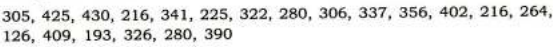
\includegraphics[]{IS/QC/4a2018.PNG} Can we conclude that the process is in control by setting up an appropriate control chart in a graph sheet.
\myline
\ques{4}{c}{15} In a single sampling plan (1000,89,2), compute the probability of acceptance of the lot if the lot fraction defective is 0.01. Also compute Average Outgoing Qulity (AOQ) of the lot.
